%\documentclass[handout,space,nooutcomes]{ximera}
\documentclass{ximera}

\graphicspath{{./}{eulerCharacteristic}}

%\usepackage[strict]{changepage}


\title{Spherical Geometry}
\author{Brad Findell \and Bart Snapp}
\begin{document}
\begin{abstract}
Here we investigate spherical geometry and compare to Euclidean (flat) geometry. 
\end{abstract}
\maketitle


%In our approach to Euclidean (i.e., flat) geometry, we make the following assumptions:
%\begin{itemize}
%\item \textbf{(A1)} Through two distinct points passes a unique line.
%\item \textbf{(A2)} Given a line and a point not on the line, there is exactly one line passing through the point which is parallel to the given line (Parallel postulate).
%\item \textbf{(A3)} The points on a line can be placed in one-to-one correspondence with the real numbers so that differences measure distances (Ruler postulate).  
%\item \textbf{(A4)} The rays with a common endpoint can be numbered so that differences measure angles and so that straight angles measure $180^\circ$ (Protractor postulate). 
%\item \textbf{(A5)} Every basic rigid motion (rotation, reflection, or translation) has the following properties:
%\begin{enumerate}
%\item It maps a line to a line, a ray to a ray, and a segment to a segment.
%\item It preserves distance and angle measure.
%\end{enumerate}
%\item \textbf{(A6)} Areas of geometric figures have the following properties: 
%\begin{enumerate}
%\item Congruent figures enclose equal areas.
%\item Area is additive, i.e., the area of the union of two regions that overlap only at their boundaries is the sum of their areas. 
%%\item Area is measured by tiling a region with a two-dimensional unit (such as a square) and parts of the unit, without gaps or overlaps. 
%\item A rectangle with side-lengths $a$ and $b$ has area $ab$, where $a$ and $b$ can be any non-negative real numbers.
%\end{enumerate}
%\end{itemize}


\section*{Getting Started}


\begin{problem}
Spherical geometry is the study of geometry on the two-dimensional surface of a sphere.  Because the surface is curved, some adjustments in language and meaning are required in order to compare and contrast with Euclidean (flat) geometry.  Most importantly, we need to decide what counts as a ``line.''

Which of the following approaches shall we take?  

\begin{multipleChoice}
\choice{Use lines tangent to the sphere.}
\choice{Use lines intersecting the sphere in two points.}
\choice[correct]{Use great circles as ``lines.''}
\choice{Use any circles as ``lines.''}
\choice{This is a fool's errand.}
\end{multipleChoice}
\begin{problem}
Correct! 

A \emph{great circle} is a circle of maximum circumference on the sphere.  The (three-dimensional) center of a great circle is the $\answer[format=string]{center}$ of the sphere itself.  Think of a great circle as the intersection of the sphere with a plane through the center of the sphere.  

\end{problem}

\end{problem}

\section*{Assumptions}
Euclidean geometry is based on assumptions about fundamental objects, such as points and lines, from which geometry is built. These assumptions are sometimes called postulates or axioms. In the following problems, we consider whether these assumptions hold in spherical geometry. 


\begin{problem} % (A1)
Euclidean assumption: Through two distinct points passes a unique line.  

Does this assumption hold in spherical geometry? 
$\answer[format=string]{no}$

\begin{problem}
%In \textbf{hyperbolic} geometry, this assumption holds. 

In \textbf{spherical} geometry, if the points are on $\answer[format=string]{opposite}$ ends of a diameter, many lines pass through both.
\begin{feedback}[correct]
\textbf{Correct!} The North and South Poles are easy examples.  
\end{feedback}
\end{problem}
\end{problem}

\begin{problem} % (A2)
Euclidean assumption: Given a line and a point not on the line, there is exactly one line passing through the point which is parallel to the given line (Parallel postulate).  

Does this assumption hold in spherical geometry? 
$\answer[format=string]{no}$
\begin{problem}
In spherical geometry, there are no parallels.  In fact, any two distinct lines intersect in $\answer{two}$ points.  

%In $\answer[format=string]{hyperbolic}$ geometry, there is more than one parallel through a point not on a line. 
\end{problem}
\end{problem}

\begin{problem} % (A3)
Euclidean assumption:  The points on a line can be placed in one-to-one correspondence with the real numbers so that differences measure distances (Ruler postulate).  

Does this assumption hold in spherical geometry? 
$\answer[format=string]{no}$

\begin{problem}
%In $\answer[format=string]{hyperbolic}$ geometry, this assumption holds. 

In spherical geometry, lines are \wordChoice{\choice[correct]{finite}\choice{infinite}} in length.  Attempting to map the real number line onto a great circle on the sphere requires ``wrapping it around'' so that many real numbers land on any point on the great circle.  
\end{problem}
\end{problem}

\begin{problem} % (A4)
Euclidean assumption:  The rays with a common endpoint can be numbered so that differences measure angles and so that straight angles measure $180^\circ$ (Protractor postulate).  

Does this assumption hold in spherical geometry? 
$\answer[format=string]{yes}$
\end{problem}

\begin{problem} % (A5)
Euclidean assumption: Every basic rigid motion (rotation, reflection, or translation) has the following properties: 
\begin{enumerate}
\item It maps a line to a line, a ray to a ray, and a segment to a segment.
\item It preserves distance and angle measure.
\end{enumerate}

Does this assumption hold in spherical geometry? 
$\answer[format=string]{yes}$
\begin{feedback}[correct]
\textbf{Correct!} But in spherical geometry, translations along a line are actually $\answer[format=string]{rotations}$ about the poles of that line.  (Think about moving a spherical transparency on a globe.) 
\end{feedback}
\end{problem}

\begin{problem} % A6
Euclidean assumption:  Areas of geometric figures have the following properties: 
\begin{enumerate}
\item Congruent figures enclose equal areas.
\item Area is additive, i.e., the area of the union of two regions that overlap only at their boundaries is the sum of their areas. 
\item A rectangle with side-lengths $a$ and $b$ has area $ab$, where $a$ and $b$ can be any non-negative real numbers.
\end{enumerate}

Does this assumption hold in spherical geometry? 
$\answer[format=string]{no}$
\begin{problem}
Rectangles (i.e., quadrilaterals with four $\answer[format=string]{right}$ angles) do not exist in spherical geometry.  %Neither do they exist in hyperbolic geometry.  

In Euclidean geometry, area can be based on tiling with unit squares.  But in spherical geometry, squares don't exist, and regular quadrilaterals don't tile the plane.
\end{problem}
\end{problem}

% Angle sum in a triangle.
% Angle sum in a quadrilateral. 

\section*{Problems}

\begin{problem}
\begin{enumerate}
\item In Euclidean geometry, the sum of the interior angles of a triangle is 
\wordChoice{\choice{less than}\choice[correct]{equal to}\choice{greater than}} 
$\answer{180}$ degrees.
\item In spherical geometry, the sum of the interior angles of a triangle is 
\wordChoice{\choice{less than}\choice{equal to}\choice[correct]{greater than}} 
$\answer{180}$ degrees.
%\item In hyperbolic geometry, the sum of the interior angles of a triangle is 
%\wordChoice{\choice[correct]{less than}\choice{equal to}\choice{greater than}} 
%$\answer{180}$ degrees.
\end{enumerate}
\end{problem}

\begin{problem}
\begin{enumerate}
\item In \emph{Euclidean} geometry, the sum of the interior angles of a quadrilateral is 
\wordChoice{\choice{less than}\choice[correct]{equal to}\choice{greater than}} 
$\answer{360}$ degrees.
\item In \textbf{spherical} geometry, the sum of the interior angles of a quadrilateral is 
\wordChoice{\choice{less than}\choice{equal to}\choice[correct]{greater than}} 
$\answer{360}$ degrees.
%\item In hyperbolic geometry, the sum of the interior angles of a quadrilateral is 
%\wordChoice{\choice[correct]{less than}\choice{equal to}\choice{greater than}} 
%$\answer{360}$ degrees.
\end{enumerate}
\end{problem}

\begin{problem} % Betweenness
In Euclidean geometry, if three distinct points are collinear, then exactly one must lie between the other two.  Does this statement hold in spherical geometry? 
$\answer[format=string]{no}$

\begin{problem}
%In $\answer[format=string]{hyperbolic}$ geometry, this assumption holds. 

In spherical geometry, lines are $\answer[format=string]{great circles}$ (two words).  So any of the three points can be seen as ``between'' the other two.  
\end{problem}
\end{problem}


%\begin{problem}
%In Euclidean geometry, a rectangle is a quadrilateral with four right angles. 
%\begin{enumerate}
%\item What can you conclude about rectangles in spherical geometries?  Explain.  
%\item What does this imply about the usefulness of familiar (Euclidean) area formulas in these other geometries?  Explain your reasoning. 
%\end{enumerate} 
%\end{problem}

%\begin{problem}
%\item In Euclidean geometry, when three distinct points $A$, $B$, and $C$, lie on a line, it is easy to tell which point is between the other two.  Does this work in spherical geometry?  Explain your reasoning.  
%\end{problem}
%

%\begin{problem}
%When walking on a sphere, how could a bug check whether she or he was traveling straight.  
%\end{problem}
%
\begin{problem}
In Euclidean geometry, given a line and a point, there is a unique perpendicular to the given line through the given point.  In spherical geometry, to what extent is this true? 
\begin{multipleChoice}
\choice{Always.}
\choice[correct]{Sometimes.}
\choice{Never.}
\end{multipleChoice}
\begin{problem}
Correct!  Most of the time such a perpendicular is unique in spherical geometry.  But if the line is the $\answer[format=string]{equator}$, there are 
\wordChoice{\choice{zero}\choice{two}\choice[correct]{infinitely many}} perpendiculars from the North Pole or the South Pole.  
\begin{problem}
In fact, every line has two ``poles'' from which there are infinitely many perpendiculars.  

Conversely, given any point on the sphere, if we imagine it to be the North Pole, there is a unique great circle corresponding to the equator, called the \emph{polar} of the point.  Any line from a point to its polar intersect the polar at $\answer[format=string]{right}$ angles.  
\end{problem} 
\end{problem} 
\end{problem}

\begin{problem}
Can the Euclidean definition of a circle make sense on a sphere?  
\begin{multipleChoice}
\choice{Yes.}
\choice[correct]{Yes, with some adjustments in interpretation.}
\choice{No.}
\end{multipleChoice}
\begin{problem}
Correct! Here is the definition:  

A circle is the set of points that are $\answer[format=string]{equidistant}$ from a given point, called the $\answer[format=string]{center}$ of the circle.  The common distance is called the $\answer[format=string]{radius}$ of the circle.  
\begin{problem}
To make sense of spherical geometry, we sometimes note that the center of a great circle is the center of the sphere and that the center of a latitude line is on the axis of the earth.  But these are $\answer[format=string]{three}$-dimensional interpretations. 

For two-dimensional geometry on the surface of a sphere, the center of a spherical circle must be a point on the $\answer[format=string]{surface}$ of the sphere.  And the radius must be measured along the $\answer[format=string]{surface}$ of the sphere (rather than as the three-dimensional shortest distance through the sphere). 

Let's use latitudes to help us make sense of spherical circles.  For reference:  At the equator, the circumference of Earth is 24,901 miles (40,075 km). From the North Pole to the South Pole, however, the circumference is slightly smaller, at 24,860 miles (40,008 km).  

Latitude $89^\circ$ is a ``small'' circle around the North Pole.  Actually, this circle has a radius of $\answer{1/360}$ (a fraction) of the circumference of the earth, which would be about $\answer[tolerance=0.5]{24860/360}$ miles.  As the radius increases, the circles move south through each of the latitudes in the Northern Hemisphere

When the radius of the spherical circle reaches $\answer{1/4}$ (a fraction) of the circumference of the sphere, the circle is in fact the equator (a great circle)---which is to say the circle becomes a line!   This circle has a maximum circumference:  If the radius of the circle continues to increase, its circumference must decrease as it proceeds into the Southern Hemisphere!  In the limiting case, when the radius is $\answer{1/2}$ (a fraction) of the circumference of the sphere, the ``circle'' has been reduced to a single point:  the South Pole.  And the circumference of this ``circle'' is $\answer{0}$. 
\end{problem}
\end{problem}
\end{problem}


% finding routes of planes or ships on the globe.  Get back to latitude lines. 

% rotations, reflections, and translations on a sphere? 

% Is radius perpendicular to tangent to circle?  

% poles of a great circle  

% perhaps compare area and circumference of the spherical and Euclidean circle.  

%  Problems about symmetries of a line on the sphere.  Use it to argue that great circles are straight.  
% Wrapping a ribbon on a sphere.    
% driving a car with fixed wheels (distance traveled). 

% antipodal points lie on opposite ends of a diameter
% lines are finite in extent
% exterior angle theorem 





\begin{problem}
On many maps of the U.S., Colorado appears to be a rectangle.  In 1861, the U. S. Congress defined the Territory of Colorado as the region from $37^\circ$N to $41^\circ$N latitude, and from $25^\circ$W to $32^\circ$W longitude, relative to the Washington Meridian.  (Today, those longitudes are from $102^\circ02'48''$W to $109^\circ02'48''$W.) 

Does this definition create a rectangle on the spherical earth?   $\answer[format=string]{no}$.

\begin{problem}
In fact, Colorado cannot be a rectangle because a quadrilateral with four right angles cannot exist on a sphere, as discussed above.  

Specifically which properties of rectangles fail?  (Select all true statements.) 

\begin{selectAll}
\choice{The eastern and western borders are not lines (i.e., great circles).}
\choice[correct]{The northern and southern borders are not lines (i.e., great circles).}
\choice{The eastern and western borders are not the same length.}
\choice[correct]{The northern and southern borders are not the same length.}
\choice{The northern angles are not right angles.}
\choice{The southern angles are not right angles.}
\end{selectAll}

\begin{problem}

Latitudes are often called ``parallels'' because any two distinct latitudes don't intersect, and they are always the same distance apart.   All latitudes are circles, and so northern and southern borders of Colorado are not straight but are arcs of circles. Furthermore, latitudes are longer closer to the equator, so the southern border of Colorado is $\answer[format=string]{longer}$ than its northern border.  

%In fact, latitude ``lines'' can be seen as concentric circles with either the North Pole or the South Pole as the common center.  But among latitudes, only the $\answer[format=string]{equator}$ is a great circle. 

Longitudes are often called meridians, and each is half of a great circle, so it is reasonable to call them longitude lines.  Longitudes are numbered as east or west of the Prime Meridian.  Longitude lines are not parallel, as they all intersect at the North and South Poles. They are farthest apart at the $\answer[format=string]{equator}$.  Longitude lines are straight.  

Latitudes run (exactly) east-west and longitudes run (exactly) north-south, so they intersect at $\answer[format=string]{right}$ angles. 

The picture below is exaggerated to give a clearer sense of the actual shape of Colorado.  And this version is flattened rather than existing on a curved surface. 

\begin{center}
\begin{tikzpicture}[line cap=round,line join=round,>=triangle 45,x=1.0cm,y=1.0cm]
\clip(-2.2,-11.2) rectangle (1.3,-8.9);
\draw [shift={(-0.6031,5.95893)},line width=1.pt]  plot[domain=4.630204927871329:4.819148280507725,variable=\t]({1.*15.044584286543115*cos(\t r)+0.*15.044584286543115*sin(\t r)},{0.*15.044584286543115*cos(\t r)+1.*15.044584286543115*sin(\t r)});
\draw [shift={(-0.6031,5.95893)},line width=1.pt]  plot[domain=4.630204927871329:4.819148280507725,variable=\t]({1.*17.016363781810142*cos(\t r)+0.*17.016363781810142*sin(\t r)},{0.*17.016363781810142*cos(\t r)+1.*17.016363781810142*sin(\t r)});
\draw [line width=1.pt] (-1.838133527688046,-9.034875672356382)-- (-2.,-11.);
\draw [line width=1.pt] (1.,-9.)-- (1.210106151732617,-10.960553437925018);
\draw (-0.4,-10.1) node[anchor=center] {Colorado};
\end{tikzpicture}
\end{center}

And below is a picture from Google Earth showing the boundary of Colorado (in yellow) along with straight lines (in purple) showing the extent to which the northern and southern borders are not straight. 

\begin{center}
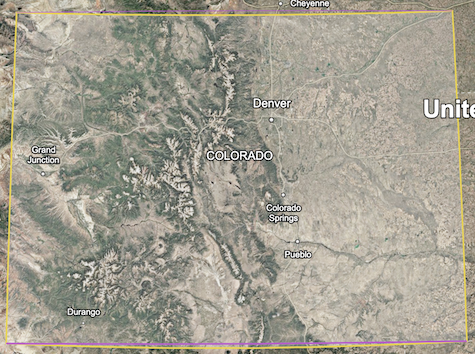
\includegraphics[scale=0.5]{colorado.png}
\end{center}

When ideal mathematics meets the real world, however, things can get messy.  When surveyors tried to carry out the congressional definition, they made mistakes.  For details, read an article \href{https://www.atlasobscura.com/articles/is-colorado-a-rectangle}{here} or \href{https://bigthink.com/strange-maps/colorado-is-not-a-rectangle/}{here}, which explains that the state is actually a polygon with $\answer{697}$ sides.  (The text of the article is the same at both links, but the graphics are different, so it is worth looking at both versions.) 


%The angle between smooth curves are defined as the angle between tangents to the curves at an intersection point.  
%
%Note: Informally, some say that a tangent touches the curve only once, but this is descriptions misleading.  For example line $k$ is a tangent to a curve $f$ at point $A$, but it intersects the curve again at point $D$.  And what about a tangent to a line?  
%
%\begin{center}
%\definecolor{uuuuuu}{rgb}{0.26666666666666666,0.26666666666666666,0.26666666666666666}
%\definecolor{qqwuqq}{rgb}{0.,0.39215686274509803,0.}
%\begin{tikzpicture}[line cap=round,line join=round,>=triangle 45,x=1.0cm,y=1.0cm]
%\begin{axis}[
%x=1.0cm,y=1.0cm,
%axis lines=middle,
%xmin=-0.8,
%xmax=7.8,
%ymin=-1.1,
%ymax=4.0,
%xtick={0.0,1.0,...,7.0},
%ytick={0.0,1.0,...,3.0},]
%\clip(-0.8,-1.1) rectangle (7.8,3.9);
%\draw[line width=1.pt,color=qqwuqq,smooth,samples=100,domain=-0.8:7.8] plot(\x,{((\x)-1)*((\x)-4)^(2)*((\x)+2)/12});
%\draw [line width=1.pt,domain=-0.8:7.8] plot(\x,{(--0.6666666666666672--0.33333333333333304*\x)/1.});
%\begin{scriptsize}
%\draw [fill=uuuuuu] (2.,1.3333333333333333) circle (1.5pt);
%\draw[color=uuuuuu] (1.86,1.63) node {$A$};
%\draw [fill=uuuuuu] (5.,2.3333333333333335) circle (1.5pt);
%\draw[color=uuuuuu] (5.22,2.15) node {$D$};
%\draw[color=uuuuuu] (4.95,3.5) node {$f$};
%\draw[color=uuuuuu] (7.4,2.9) node {$k$};
%\end{scriptsize}
%\end{axis}
%\end{tikzpicture}
%\end{center}
%
%In calculus, a tangent is defined as a line through two points ``infinitely close’’ to each other on the curve.  Intuitively, we can imagine zooming in close enough so that the curve appears straight.  Then we see that points far away are not relevant.  And it becomes clear that a tangent to a line is the line itself.  
%
%Then, a radius of a circle is perpendicular to the circle.  



\end{problem}

\end{problem}

\end{problem}

\begin{problem}
A bear goes traveling.  She walks due south for one mile, turns left $90^\circ$, and walks due east for one mile.  She again turns left $90^\circ$, and then walks due north for one mile, ending in the place where she started.  What color is the bear?  $\answer[format=string]{white}.$

Explain your reasoning.  
\begin{hint}
Where on earth could the bear be?  
\end{hint}

\begin{problem}
Correct!  The bear is white because she starts at the $\answer[format=string]{North Pole}$ (two words).  Traveling due south and due north, must be along 
$\answer[format=string]{longitude}$ lines are straight paths.  Traveling due east must be at constant $\answer[format=string]{latitude}$, which requires a circular path.  
\begin{center}
\definecolor{xdxdff}{rgb}{0.49019607843137253,0.49019607843137253,1.}
\begin{tikzpicture}[line cap=round,line join=round,>=triangle 45,x=1.0cm,y=1.0cm]
\clip(-1.7,-3.4) rectangle (1.77,0.5);
\draw [shift={(0.,0.)},line width=1.pt]  plot[domain=4.21238898038469:5.21238898038469,variable=\t]({1.*2.9955555555555518*cos(\t r)+0.*2.9955555555555518*sin(\t r)},{0.*2.9955555555555518*cos(\t r)+1.*2.9955555555555518*sin(\t r)});
\draw [line width=1.pt] (0.,0.)-- (-1.4361458356410335,-2.62884731872938);
\draw [line width=1.pt] (0.,0.)-- (1.4361458356410333,-2.62884731872938);
\draw [-stealth,line width=1.pt] (-0.57,-0.55) -- (-1.22,-1.73);
\draw [-stealth,line width=1.pt] (1.22,-1.73) -- (0.57,-0.55);
\draw [-stealth,line width=1.pt] (-0.50,-3.2) -- (0.5,-3.2);
\draw [fill=xdxdff] (0.,0.) circle (1.5pt);
\draw[color=xdxdff] (0.1,0.3) node {$N$};
\end{tikzpicture}
\end{center}
\end{problem}
\end{problem}

\end{document}
